\chapter{Cinematica}

    \section{Moto rettilineo uniforme}

        \paragraph{Velocità} 
            La velocità viene rappresentata da uno scalare:
            \begin{equation}
                v_x = k \; [m/s]
            \end{equation}

        \paragraph{Velocità media} 
            La velocità media viene rappresentata come un intervallo di uno 
            spostamento su un intervallo di tempo:
            \begin{equation}
                v_m = \frac{\Delta x}{\Delta t} = \frac{x_f - x_i}{t_f - t_i}
            \end{equation}

        \paragraph{Velocità istantanea} detta anche semplicemente velocità di 
        una particella, è definita come:
            \begin{equation}
                v = \lim_{x \to 0}  \frac{\Delta x}{\Delta t} = \frac{dx}{dt}
            \end{equation}

        \paragraph{Spostamento}
            \begin{equation}
                x(t) = x_i + v_xt \; [m]
            \end{equation}

    \section{Moto uniformemente accelerato}

        \paragraph{Accelerazione media} è il rapporto fra la variazione della
        velocità $\Delta v$ che avviene in un intervallo di tempo $\Delta t$, 
        definita come:
        \begin{equation}
            a_m = \frac{\Delta v}{\Delta t} = \frac{v_f - v_i}{t_f - t_i} 
            \, [m/s^2]
        \end{equation}

        \paragraph{Accelerazione istantanea} o semplicemente accelerazione, è 
        la rapidità di variazione della velocità. Matematicamente si tratta 
        della derivata seconda della posizione $x(t)$ rispetto al tempo:
        \begin{equation}
            a = \frac{dv}{dt} = \frac{d^2x}{dt^2}
        \end{equation}

        \paragraph{Spostamento}
            \begin{equation}
                x(t) = x_i + v_it + \frac{1}{2}at^2 \; [m]
            \end{equation}

        \paragraph{Velocità finale}
            \begin{equation}
                v_f(t) = v_{i} + at
            \end{equation}
    
        \paragraph{Caso particolare}
            Per determinare il tempo possiamo effettuare la formula inversa 
            dello spostamento. È possibile notare come il tempo non dipende 
            dalla massa degli oggetti, ma dall'altezza e dalla forza di gravità
            . In assenza d'aria di conseguenza due oggetti con masse 
            completamente diverse arrivano a terra allo stesso tempo!

            \begin{equation}
                t_c=\sqrt{\frac{2h}{g}} \; [s]
            \end{equation}

    \section{Moto di un proiettile} 

        Il moto di un proiettile è scomponibile lungo gli assi cartesiani in 
        due moti ben distinti, agenti su un unico corpo:
        \begin{itemize}
            \item \textbf{Asse X}: moto rettilineo uniforme.
            \item \textbf{Asse Y}: moto rettilineo uniformemente accelerato.
        \end{itemize}
        Soffermandoci su questo ragionamento possiamo notare come la forza di 
        gravità (accelerazione) agisca in modo costante lungo l'asse y 
        effettuando un'accelerazione negativa (decelerazione) lungo questa 
        componente del moto. Il moto dell'asse x invece non viene intaccato da 
        nessun'altra forza (trascurando ovviamente l'attrito dell'aria).
        
        \paragraph{Equazioni del moto}
        (Per assi cartesiani)
        \begin{align}
            \textsf{Moto} &: \begin{cases}
                    x(t) &= x_0 + v_{0x}t \\
                    y(t) &= y_0 + v_{0y}t + \frac{1}{2}at^2
                \end{cases} \\
                \textsf{Velocità} &: v_{f} = v_{0} + at
        \end{align}

    \section{Moto circolare uniforme}
        Nel moto circolare uniforme agiscono 3 forze:
        \begin{itemize}
            \item Velocità tangenziale
            \item Accelerazione centripeta
            \item Accelerazione centrifuga
        \end{itemize}
        Le prime due sono forze fisiche reali, mentre la terza è chiamata forza
        apparente. Difatti la forza che ci fa sentire spinti verso l'esterno è
        data dalla nostra inerzia nel tendere a proseguire il nostro moto 
        diritti, mentre l'accelerazione centripeta (sempre rivolta verso il
        centro della curva) ci tiene in traiettoria circolare. Questo accade
        perché ci troviamo in un sistema non inerziale: difatto se lanciassimo 
        una pallina mentre ci troviamo all'interno di un moto circolare essa ci
        sembrerà allontanarsi da noi con una sua traiettoria, spinta da una 
        forza (apparente) verso l'esterno. Vista da un osservatore posto al di
        fuori del moto (in un sistema inerziale) semplicemente la pallina 
        proseguirà diritta nella sua traiettoria.\\\\
        Analizziamo ora le formule del moto circolare uniforme:

        \paragraph{Velocità tangenziale} La velocità tangenziale è lo spazio 
        percorso dal punto materiale in un intervallo di tempo:
        \begin{equation}
            v = \frac{2\pi r}{T} \; [m/s]
        \end{equation}

        \paragraph{Accelerazione centripeta} L'accelerazione centripeta è 
        quella forza che mantiene un corpo in un moto circolare uniforme. Essa
        è sempre diretta verso il centro della circonferenza!.
        \begin{equation}
            a_c = \frac{v^2}{r} \; [m/s^2]
        \end{equation}
        Come vedremo più avanti in questo formulario l'accelerazione è impressa
        da una forza agente sul corpo, descrivibile (tramite la Seconda Legge
        di Newton) come:
        \begin{equation}
            F_{accelerazione} = ma = m\frac{v^2}{r} \, \Bigg[N = 
            \frac{Kg \cdot m}{s^2} \Bigg]
        \end{equation}

        \paragraph{Periodo} Il tempo richiesto perché una particella completi
        una circonferenza è:
        \begin{equation}
            T = \frac{2\pi r}{v} \;
        \end{equation}

        \paragraph{Velocità angolare} La velocità angolare è l'angolo percorso
        dal punto materiale in un intervallo di tempo:
        \begin{equation}
            \omega = \frac{2\pi}{T} \, \Bigg[\frac{rad}{s} \Bigg]
        \end{equation}
        Espressa in radianti al secondo.

    
        \subsection{Moto Armonico}  \label{moto_armonico}
        Il moto circolare uniforme può essere scomposto in due moti sinusoidali 
        $\sin$ e $\cos$.
        Il moto circolare uniforme e quello uniformemente accelerato possono 
        essere perfettamente paragonati al moto rettilineo uniforme e quello 
        uniformemente accelerato. In questo caso $\Theta$ è la nostra $x$ 
        mentre la velocità $v$ diventa $\omega$.\\\\
        Nel caso uniformemente accelerato l'accelerazione $a$ diventa $\alpha$.

        \paragraph{Legge oraria (equazione del moto)} Essa descrive il moto del
        moto circolare uniforme, espresso come angolo in funzione del tempo:
        \begin{equation}
            \Theta = \Theta_0 + \omega t = 
            \begin{cases}
                x(t)=R\cos{\Theta(t)} \\
                y(t)=R\sin{\Theta(t)}
            \end{cases} 
            = 
            \begin{cases}
                x(t)=R\cos{(\Theta_o+\omega t)} \\
                y(t)=R\sin{(\Theta_o+\omega t)}
            \end{cases}
        \end{equation}

        \paragraph{Velocità tangenziale} La velocità tangenziale è lo spazio 
        percorso dal punto materiale in un intervallo di tempo:
        \begin{equation}
            v = \frac{2\pi r}{T} = 
            \begin{cases}
                v_x=-R\omega\sin{(\Theta_o+\omega t)} \\
                v_y=R\omega\cos{(\Theta_o+\omega t)}
            \end{cases}
        \end{equation}

        \begin{quote}
            Da notare come (per definizione) le equazioni della velocità non 
            sono altro che la derivata ' dell'equazione del moto 
            (Legge oraria)! 
        \end{quote}

        \paragraph{Accelerazione centripeta} L'accelerazione centripeta è 
        quella forza che mantiene un corpo in un moto circolare uniforme. Essa
        è sempre diretta verso il centro della circonferenza!.
        \begin{equation}
            a_c = \frac{v^2}{r}=
            \begin{cases}
                a_x=-R\omega^2\cos{(\Theta_o+\omega t)} \\
                a_Y=-R\omega^2\sin{(\Theta_o+\omega t)}\end{cases}
        \end{equation}

        \begin{quote}
            Da notare come (per definizione) le equazioni dell'accelerazione 
            non sono altro che la derivata " dell'equazione del moto 
            (Legge oraria)! 
        \end{quote}
        
    \section{Moto circolare uniformemente accelerato} Nel moto circolare 
    uniformemente accelerato entra in gioco l'accelerazione totale come somma
    vettoriale dell'accelerazione centripeta e dell'accelerazione tangeziale.
    Di conseguenza l'equazione del moto sarà il sistema:

        \paragraph{Legge oraria (equazione del moto)}
        \begin{equation}
            \begin{cases} 
                \Theta = \Theta_0 + \omega_0t + \frac{1}{2}\alpha t^2 \\ 
                \omega = \omega_0+\alpha t
            \end{cases}
        \end{equation}

        \subsection{Tabelle di riepilogo} Di seguito sono riportate due tabelle 
        contententi un riepilogo delle formule (comprese le formule inverse) 
        sia del Moto circolare uniforme \ref{fig:MCU} che del Moto circolare 
        uniformemente accelerato \ref{fig:MCUA}.

        \begin{figure}[H]
            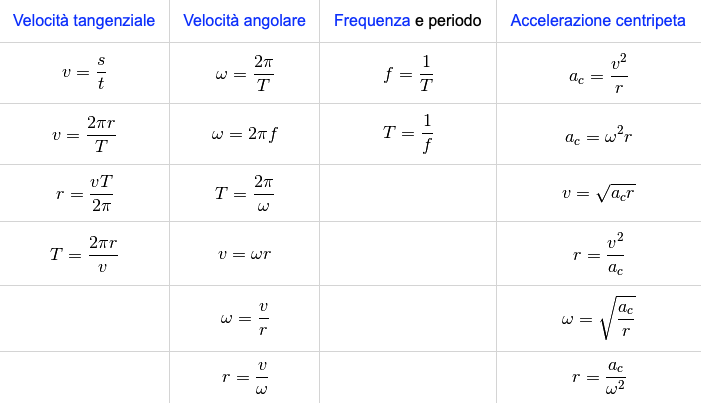
\includegraphics[width=0.9\linewidth]
            {formulario/img/Formulario_MCU.png}
            \caption{Formule del Moto circolare uniforme}
            \label{fig:MCU}
        \end{figure}

        \begin{figure}[H]
            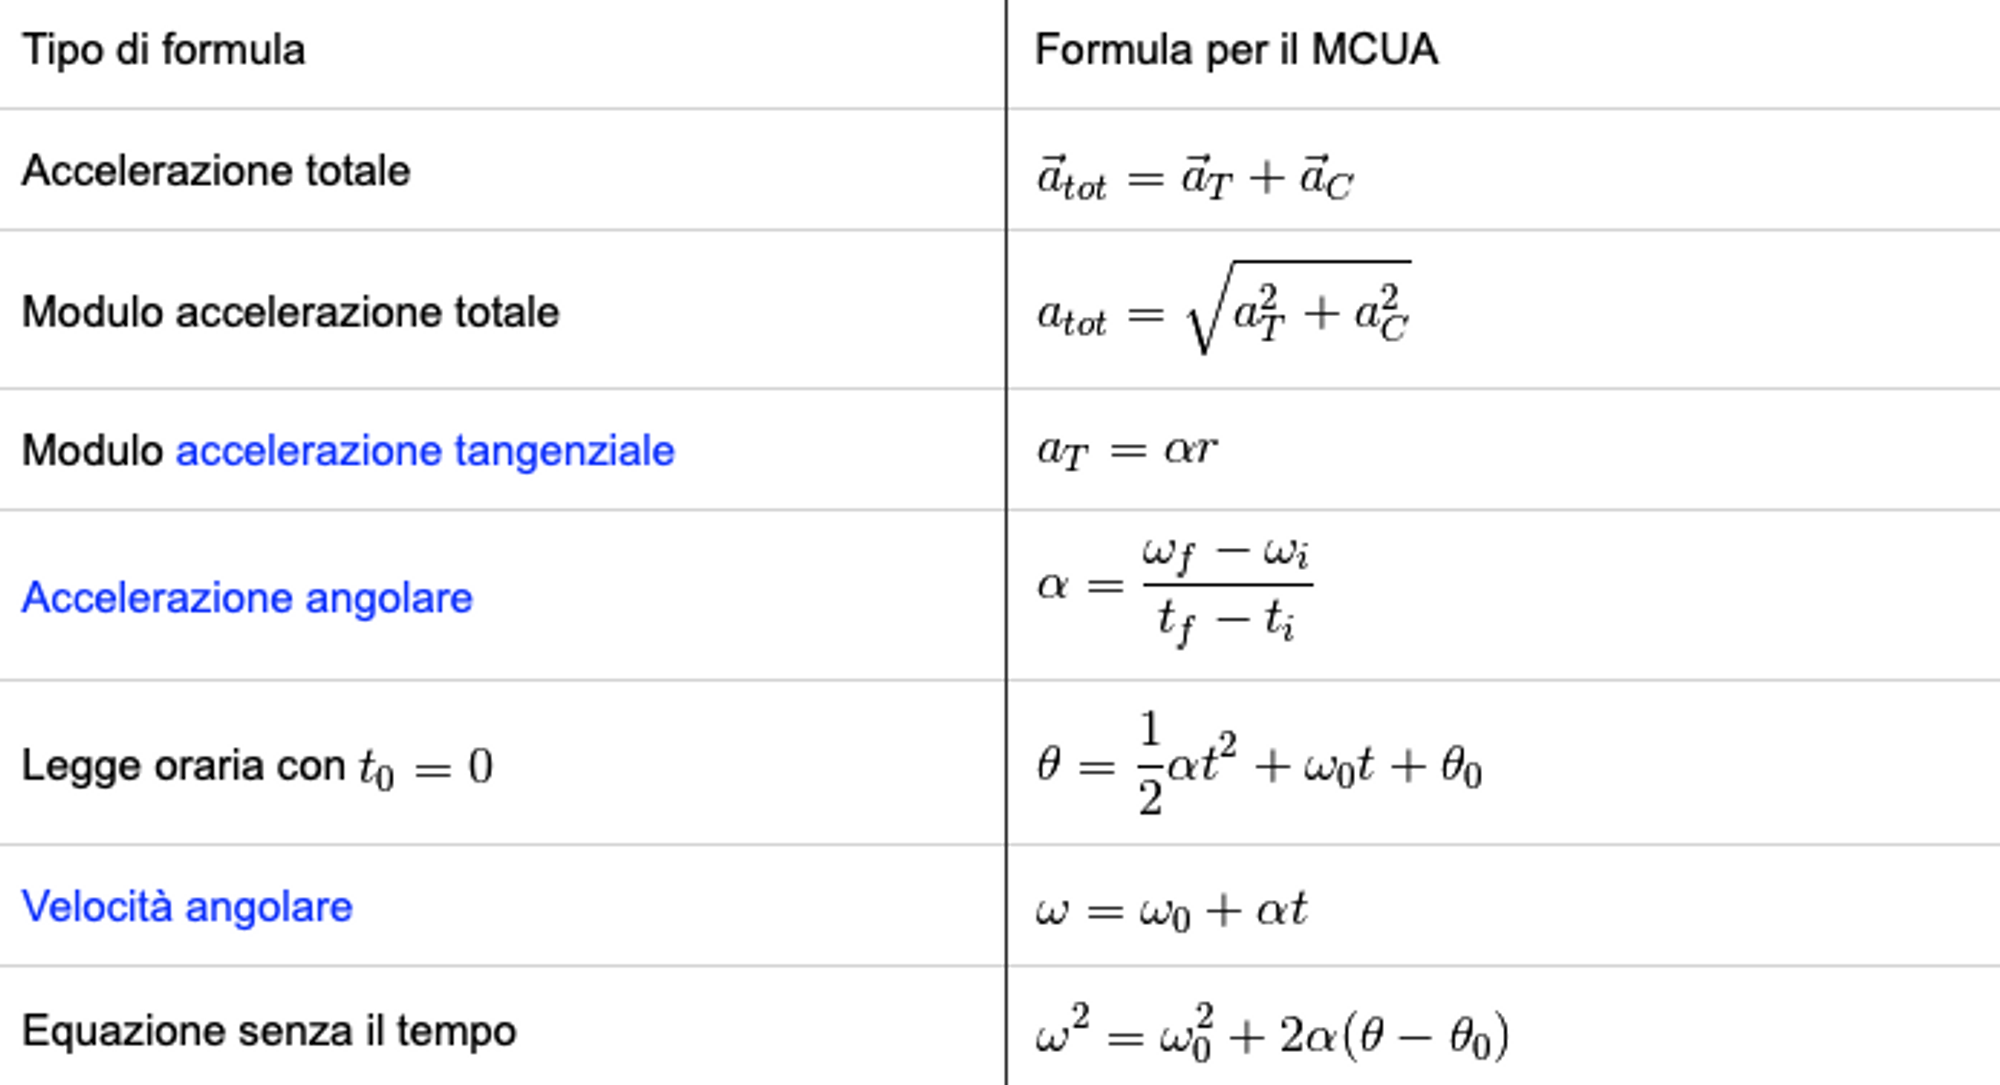
\includegraphics[width=0.9\linewidth]
            {formulario/img/Formulario_MCUA.png}
            \caption{Formule del Moto circolare uniformemente accelerato}
            \label{fig:MCUA}
        \end{figure}

        